
\begin{frame}{Zum Aufwärmen: Vogelfarben}
	Wir zeigen nun:\\[2em]
	{\LARGE
	Alle Vögel haben die gleiche Farbe!}\\
	\bigskip
	\only<beamer:0>{Achtung: Dieser Beweis ist natürlich \textbf{kaputt}!}
\end{frame}

\begin{frame}[t]{Zum Aufwärmen: Vogelfarben}
	\only<1|handout:1>{
		Das machen wir mit \textbf{vollständiger Induktion} und zeigen die folgende, äquivalente Aussage: \\
	}
	
	\only<1-3|handout:1-2>{
		\[
			\begin{array}{r@{\ }l}
			\forall n \in \N_+ : &\text{ In jeder Menge, die genau } n \text{ Vögel enthält,} \\
								 &\text{ haben alle Vögel die gleiche Farbe.}
			\end{array}
		\]
		
	}
	
	\only<2-3|handout:2>{	
		\begin{block}{Induktionsanfang}
			$n = 1$: Wenn eine Menge genau einen Vogel enthält, dann haben
			offensichtlich alle Vögel die gleiche Farbe. \textbf{\checked}
		\end{block}
	}
	\only<3|handout:2>{
		\begin{block}{Induktionsvoraussetzung}
			Für ein beliebiges aber festes $n$ gelte: In jeder
			Menge, die genau $n$ Vögel enthält, haben alle Vögel die gleiche Farbe.
		\end{block}
	}

	\only<4-5|handout:3-4> {
	\begin{block}{Induktionsschritt}
		\only<4|handout:3>{
			Wir zeigen die Aussage für $n+1$: Sei also $M$ eine Menge,
			die genau $n+1$ Vögel enthalte. Wir stellen uns vor, dass die Vögel
			alle nebeneinander sitzen:
		}
	
		\begin{figure}
			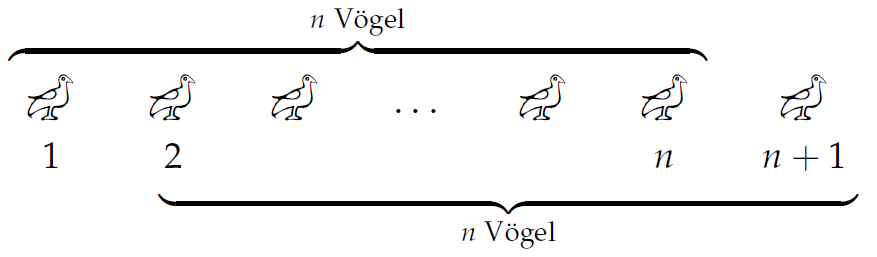
\includegraphics[scale=0.4]{induktion_voegel}
			\centering
		\end{figure}
	
		\only<5|handout:4>{
			Die Vögel $1, 2, ..., n$ bilden eine Menge mit genau $n$ Vögeln. Also haben sie nach IV alle die gleiche Farbe.\\ 
			Die Vögel $2, 3, ..., n + 1$ bilden auch eine Menge mit genau $n$ Vögeln. Also haben nach IV auch diese alle die gleiche Farbe.\\
			Damit haben auch die Vögel $1$ und $n + 1$ die gleiche Farbe, also haben alle Vögel die gleiche Farbe. $\qed$
		}
	\end{block}
	}
\end{frame}

\begin{frame}[t]{Vogelfarben: Auflösung}
	\begin{block}{Was geht schief?}
		\begin{figure}
			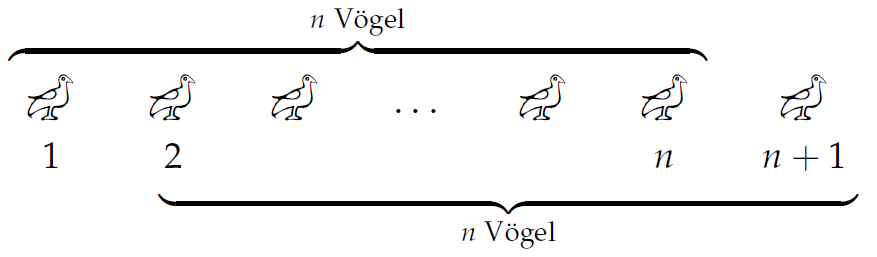
\includegraphics[scale=0.4]{induktion_voegel}
			\centering
		\end{figure}
		\pause
		Hübsches Bild. Scheint sauber. Ist bloß für $n=2$ völlig kaputt, die beiden Teilmengen \textbf{überlappen sich} dann nämlich \textbf{nicht}. \\
		\impl Wir können nicht sagen, dass der erste und letzte Vogel immer die gleiche Farbe haben. (Und wenn schon zwei Vögel nicht immer die gleiche Farbe haben, dann drei etc. auch nicht.) \\
		\impl Ganze Induktion \textbf{kaputt}. \frownie
	\end{block}	
	%Das Bild ist zwar außerordentlich hübsch, suggeriert aber leider etwas, was nicht immer stimmt: Für $n = 2$ überlappen sich die Teilmengen „ohne den ersten“ und „ohne den letzten“ Vogel nicht. Es ist also nicht erzwungen, dass beide Vögel die gleiche Farbe haben. (Und das macht „alles weitere“ auch kaputt: Wenn nicht immer 2 Vögel die gleiche Farbe haben, dann auch nicht immer 3 Vögel, usw.)
\end{frame}